\chapter{Metodologia}
\label{cap:metodologia}
O sistema proposto neste projeto, se refere a uma plataforma que fornece tanto os dispositivos para a captação dos dados dos imunobiológicos, quanto ao sistema em nuvem para armazenagem dos dados e de um aplicativo móvel para a gerência e análise das informações, seguindo a mesma estrutura representada na figura \ref{fig:end-nodes-gateways} na sessão \ref{fund:lora}, de modo a fornecer aos usuários, um produto  de fácil uso para monitorização de temperatura e umidade, possibilitando o histórico dos dados coletados em um determinado cliente.

Podemos então, separar este sistema em quatro partes, cada uma delas com uma determinada função, elas são, end-node, gateway, servidor e aplicativo móvel. Mas antes, para uma visão geral, vamos ver como foi estruturado o envio de pacotes entre cada etapa.

% ---
\section{Estrutura dos Pacotes}
\label{metod:pacotes}
Definir um padrão de transmissão dos pacotes é de suma importância para facilitar a identificação dos dados e ajuda no reconhecimento de possíveis erros que possam ocorrer na transmissão dos dados.

Dentre a comunicação do gateway, servidor e o aplicativo móvel, que utiliza o protocolo HTTP, existem vários padrões de transmitir dados já definidos e consolidados pela comunidade,  um dos mais utilizados é o \textit{JavaScript Object Notation}, JSON, um formato leve e de código aberto, se baseando na estrutura de objetos do JavaScript.

Entretanto, o JSON é considerado uma formato leve para o HTTP e seu ecossistema, para o LoRa, que tem um limite bem menor de dados para ser transmitido, é preciso utilizar outro padrão. Para isto, optamos pelo simples, transmitir os dados separando-os pelo caractere ponto e vírgula, na seguinte ordem: temperatura, umidade, identificador do end node e o contador de pacotes transmitidos.

% ---
\section{End Node}
\label{metod:node}
O end node é o hardware que fica dentro dos ambientes de armazenagem coletando os dados de temperatura e umidade e enviado para o gateway. Para o melhor entendimento podemos separá-lo em três partes, o sensor, o transceptor LoRa e o microcontrolador, como pode ser visto na figura \ref{fig:end-node-schematic}.

\begin{figure}[H]
  \centering
  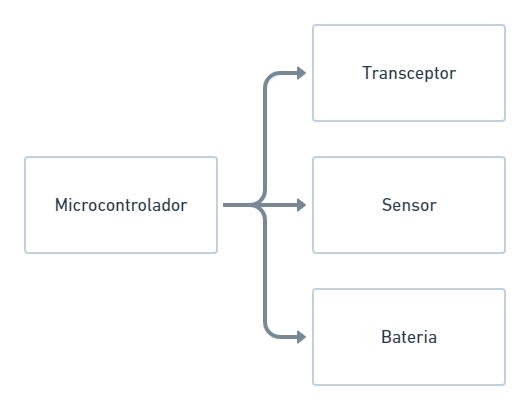
\includegraphics[width=.80\textwidth]{assets/end-node-schematic.png} 
  \caption{Representação da conexão entre os componentes principais do end node (autoral).}
  \label{fig:end-node-schematic} 
\end{figure}

Dentre os diversos sensores disponíveis no mercado para monitoramento de temperatura e umidade, optou-se por escolher um sensor da família DHT, pois é bastante difundida na comunidade, tendo uma boa relação custo benefício. Entre esses sensores, aderimos por usar o DHT22, que consegue captar a temperatura e umidade do ambiente dentro das faixas necessárias para o projeto, com uma boa precisão.

Para o microcontrolador, foi escolhido usar um ATmega328, pois é o utilizado na maioria dos Arduinos, o que nos trás dois grandes benefícios, poder utilizar um arduino como protótipo inicial, por ser fácil de encontrar, de programar e para um protótipo secundário, utilizando o microcontrolador sem o Arduino em si, ainda é possível utilizar o mesmo código, bibliotecas e o mesmo Ambiente de desenvolvimento integrado, IDE, utilizado no primeiro protótipo.

Entre os modelos de transceptores LoRa, o eleito foi o RFM95W, por ser o modelo mais simples e com menos custo e por ser o utilizado dentro do \textit{shield} Arduino, um componente modular feito para adicionar novas funcionalidades a um Arduino de forma fácil e prática, facilitando assim, o desenvolvimento do primeiro protótipo.

Em relação à alimentação do protótipo, é um ponto mais complicado de se analisar e ter uma escolha realmente boa para o caso, mesmo fazendo uma análise aprofundada, apenas teremos uma aproximação da sua eficiência, tal processo é melhor detalhado na seção \ref{metod:end-node:bateria}.

% ---
\subsection{Primeiro Protótipo}
\label{metod:end-node:1-proto}
O primeiro protótipo foi feio com o objetivo de validar os usos das tecnologias, seu alcance, e sua competência em relação a interferências ao longo do trajeto. O consumo energético foi deixado de lado neste protótipo, pois foi utilizado o Arduino e ele possui muitos componentes desnecessários para esta aplicação, que acabam aumentando o gasto energético do dispositivo.

Ele coleta os dando utilizando o sensor DHT-22, formata os dados em uma string e o envia através do LoRa, após isto, ele entra em modo de sono profundo (deep sleep) para economizar bateria por um determinado tempo, ao acordar, ele realiza a medição novamente, e fica nesse ciclo.

\begin{figure}[H]
  \centering
  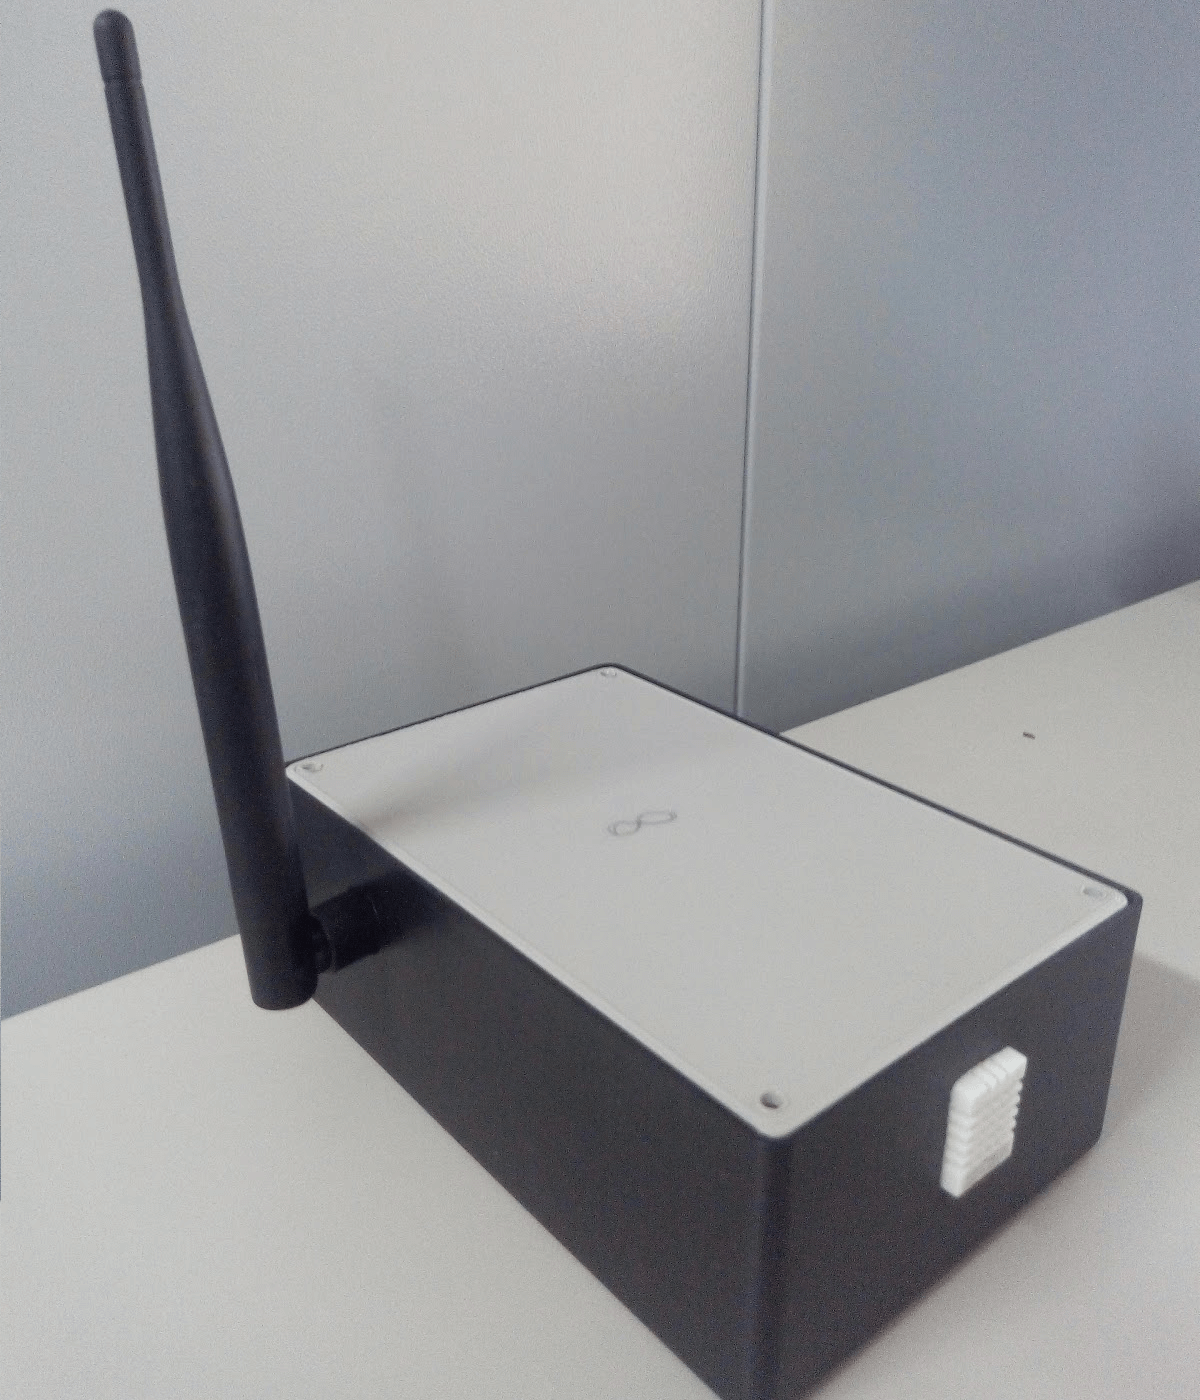
\includegraphics[width=.80\textwidth]{assets/end-node-proto-1.png} 
  \caption{Foto do primeiro protótipo (autoral).}
  \label{fig:end-node-proto-1} 
\end{figure}

% ---
\subsection{Segundo Protótipo}
\label{metod:end-node:2-proto}
O objetivo na construção deste protótipo é construir um dispositivo com um tamanho reduzido e melhorar sua eficiência energética, visando o seu funcionamento por meses com apenas uma pequena bateria. Para conseguir alcançar tais metas, é preciso remover as partes desnecessárias para o funcionamento da aplicação pelo Arduino. Pegando apenas os componentes essenciais, microcontrolador Atmega328, transceptor LoRa RFM95W e o sensor DHT-22, junto com alguns componentes de suporte para fornecer o funcionamento correto, um capacitor de cerâmica de 100pF, dois resistores de 10k Ohms  e um circuito para fornecer o clock para o microcontrolador composto por um cristal oscilador de 16mhz e dois capacitores de cerâmica de 22pF. Tal circuito, como pode ser visto na figura \ref{fig:end-node-proto-2}, foi montado em uma protoboard junto com um conversor USB para serial, para ser possível ver os logs do dispositivo pelo computador.

\begin{figure}[H]
  \centering
  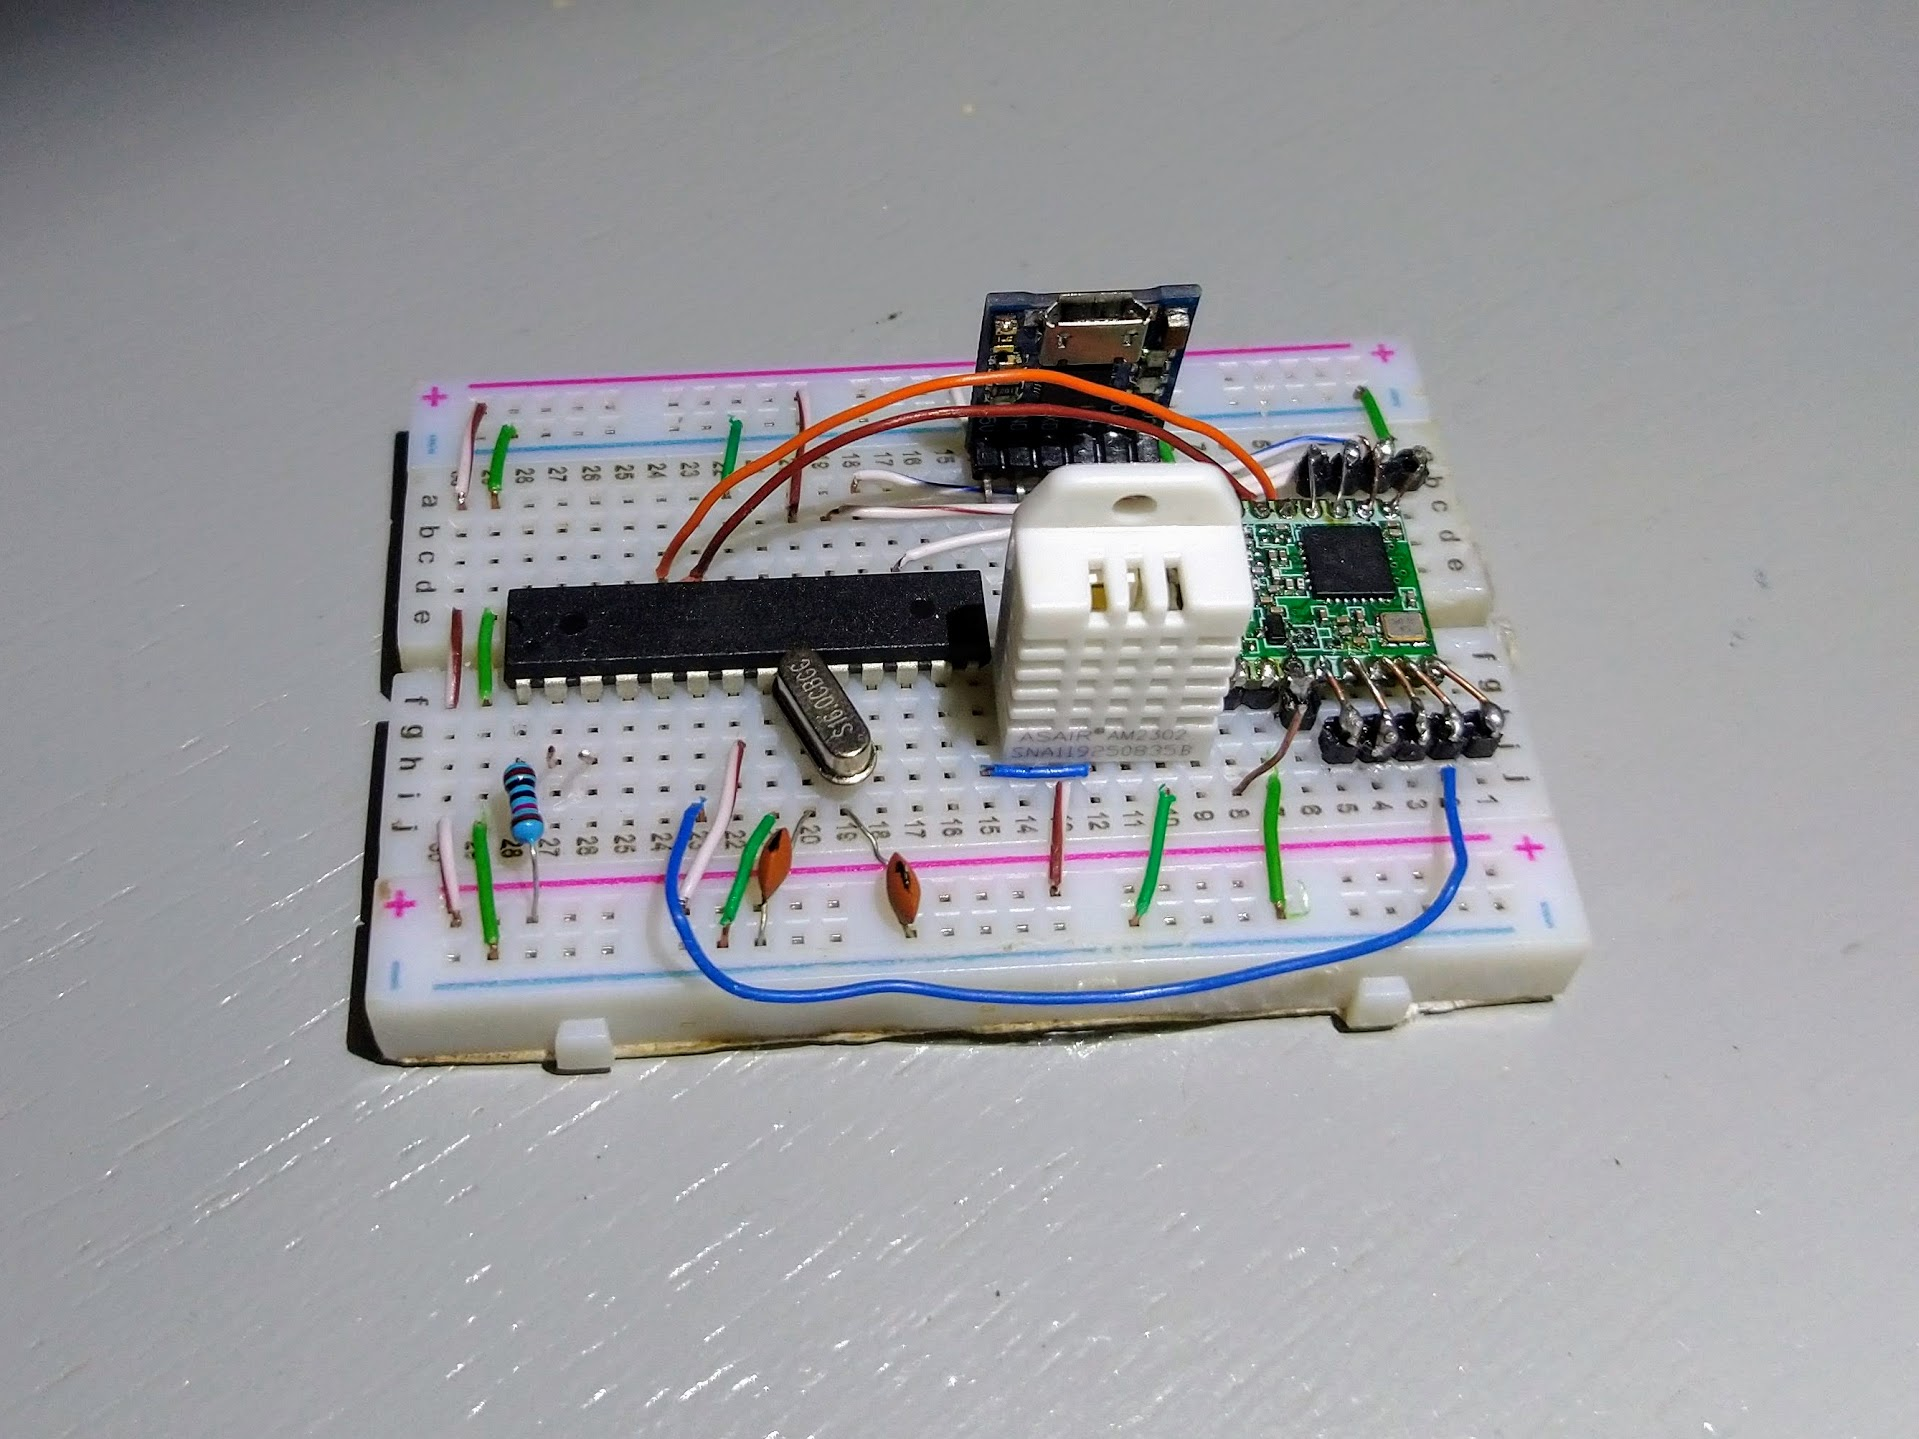
\includegraphics[width=.80\textwidth]{assets/end-node-proto-2.png} 
  \caption{Foto do segundo protótipo (autoral).}
  \label{fig:end-node-proto-2} 
\end{figure}

% ---
\subsection{Escolha da Bateria}
\label{metod:end-node:bateria}
A parte crucial a ser analisada é o consumo de energia, isso é importante para a escolha correta da bateria, que levará a uma duração aceitável do circuito que pode ser meses até anos dependendo da necessidade do produto. É preciso ter em mente as tensões de trabalho dos componentes principais da aplicação, para assim ser possível analisar qual deve ser o valor ideal de trabalho do dispositivo, é possível ver tal informação na tabela \ref{tab:end-node-componentes-volts}, mostrando a tensão mínima e máxima do microcontrolador, transceptor e sensor. Com isto, podemos ver que a tensão de limite superior do dispositivo é referente ao do transceptor LoRa, que funciona até 3,7 Volts, e a tensão de limite inferior, é a do sensor DHT-22, que equivale a 3,3 Volts, se utilizar uma tensão fora deixa faixa, o dispositivo não funcionará corretamente. 

A ideia inicial antes da análise era de usar duas pilhas AA convencionais, entretanto após a análise, tal opção torna-se inviável, pois a tensão máxima de duas baterias AA equivale a 3 Volts, o que é menos do que o mínimo necessário para o sensor DHT-22 funcionar.

\begin{table}[H]
\centering 
\scalebox{1} {
	\begin{tabular}{l | l}
	\textbf{Componente}&\textbf{Tensão de trabalho}\\[5pt] \hline
  \\
	ATmega328&2,7V até 5,5V\\[5pt]
	LoRa RFM95W&1,8V até 3,7V\\[5pt]
	DHT-22&3,3V até 5,5V\\[5pt]
	\end{tabular}
}
\caption{tensão de trabalho dos componentes principais do protótipo (autoral).}
\label{tab:end-node-componentes-volts}
\end{table}

Depois de algumas pesquisas, nos deparamos com uma bateria genérica de referência 18650, que tem o mesmo tamanho de uma AA, é fácil de encontrar em lojas de eletrônica, tem uma capacidade que varia entre 2200mAh e 3400mAh conforme o fabricante, e o mais importante, tem a tensão nominal de 3.7 Volts, o máximo que nosso circuito suporta. Sabendo que os ambientes de armazenagens de vacinas ficaram em torno de -5°C a 8°C, na figura \ref{fig:battery-discharge} podemos ver a linha de descarga da bateria conforme a temperatura de funcionamento, para simplificar os cálculos podemos usar a linha em azul de 0°C. nossa tensão de corte é de 3.3 Volts, analisando o gráfico vemos que a bateria em um ambiente a 0°C a capacidade da bateria cai para aproximadamente 90\%, que equivale há 1980mAh do modelo de 2200mAh.

\begin{figure}[H]
  \centering
  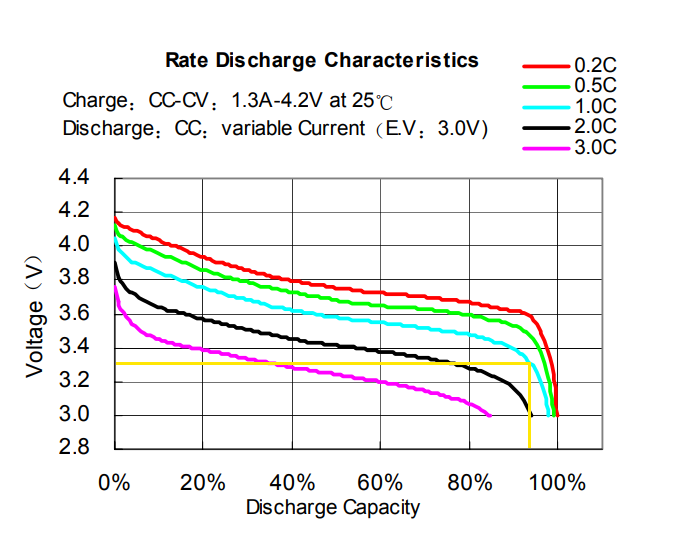
\includegraphics[width=.80\textwidth]{assets/18650-discharge.png} 
  \caption{Descarga da bateria 18650 conforme a temperatura do ambiente (Adaptada de \cite{EEMB201018650}).}
  \label{fig:battery-discharge} 
\end{figure}

% ---
\section{Gateway}
\label{metod:gateway}
O gateway é o dispositivo que fica entre os end nodes e o servidor, e em cada um desses lados, é utilizado uma tecnologia de comunicação diferente, para receber os dados enviados pelos end nodes, se utiliza o LoRa, já para enviar estes dados para o servidor, utiliza-se o HTTP via WiFi. Por isso, é preciso que o gateway possua essas duas tecnologias nele. Felizmente, a Heltec Automation, uma empresa que desenvolve produtos voltada para a IoT utilizando o LoRa, possui um microcontrolador ESP32 que contém tanto o transceptor LoRa, quanto o WiFi, como podemos ver na figura \ref{fig:esp32-lora}. Para programá-lo, foi utilizado a linguagem Arduino, compartilhando assim, a mesma biblioteca entre o end node e o gateway, para o manuseio do transceptor LoRa.

Seu funcionamento segue a seguinte linha, ele fica no aguardo dos pacotes dos end nodes, ao receber um, é realizado uma análise de erro simples, onde é verificado se a formatação do pacote está como esperado, se for detectado algum erro de formatação é enviado para o servidor os valores do RSSI, SNR, o contador do pacote e um atributo booleano marcado como falso, indicando que veio com erro para a seguinte rota, \textit{/packages/:endnodeId}, onde \textit{:endnodeId} é substituído pelo identificador do end node recebido pelo gateway. Se nenhum erro foi detectado, é enviado para a rota do servidor \textit{/sensors/:endnodeId}, os mesmo dados de RSSI, SNR e contador do pacote com o acréscimo dos dados de temperatura e umidade.

\begin{figure}[H]
  \centering
  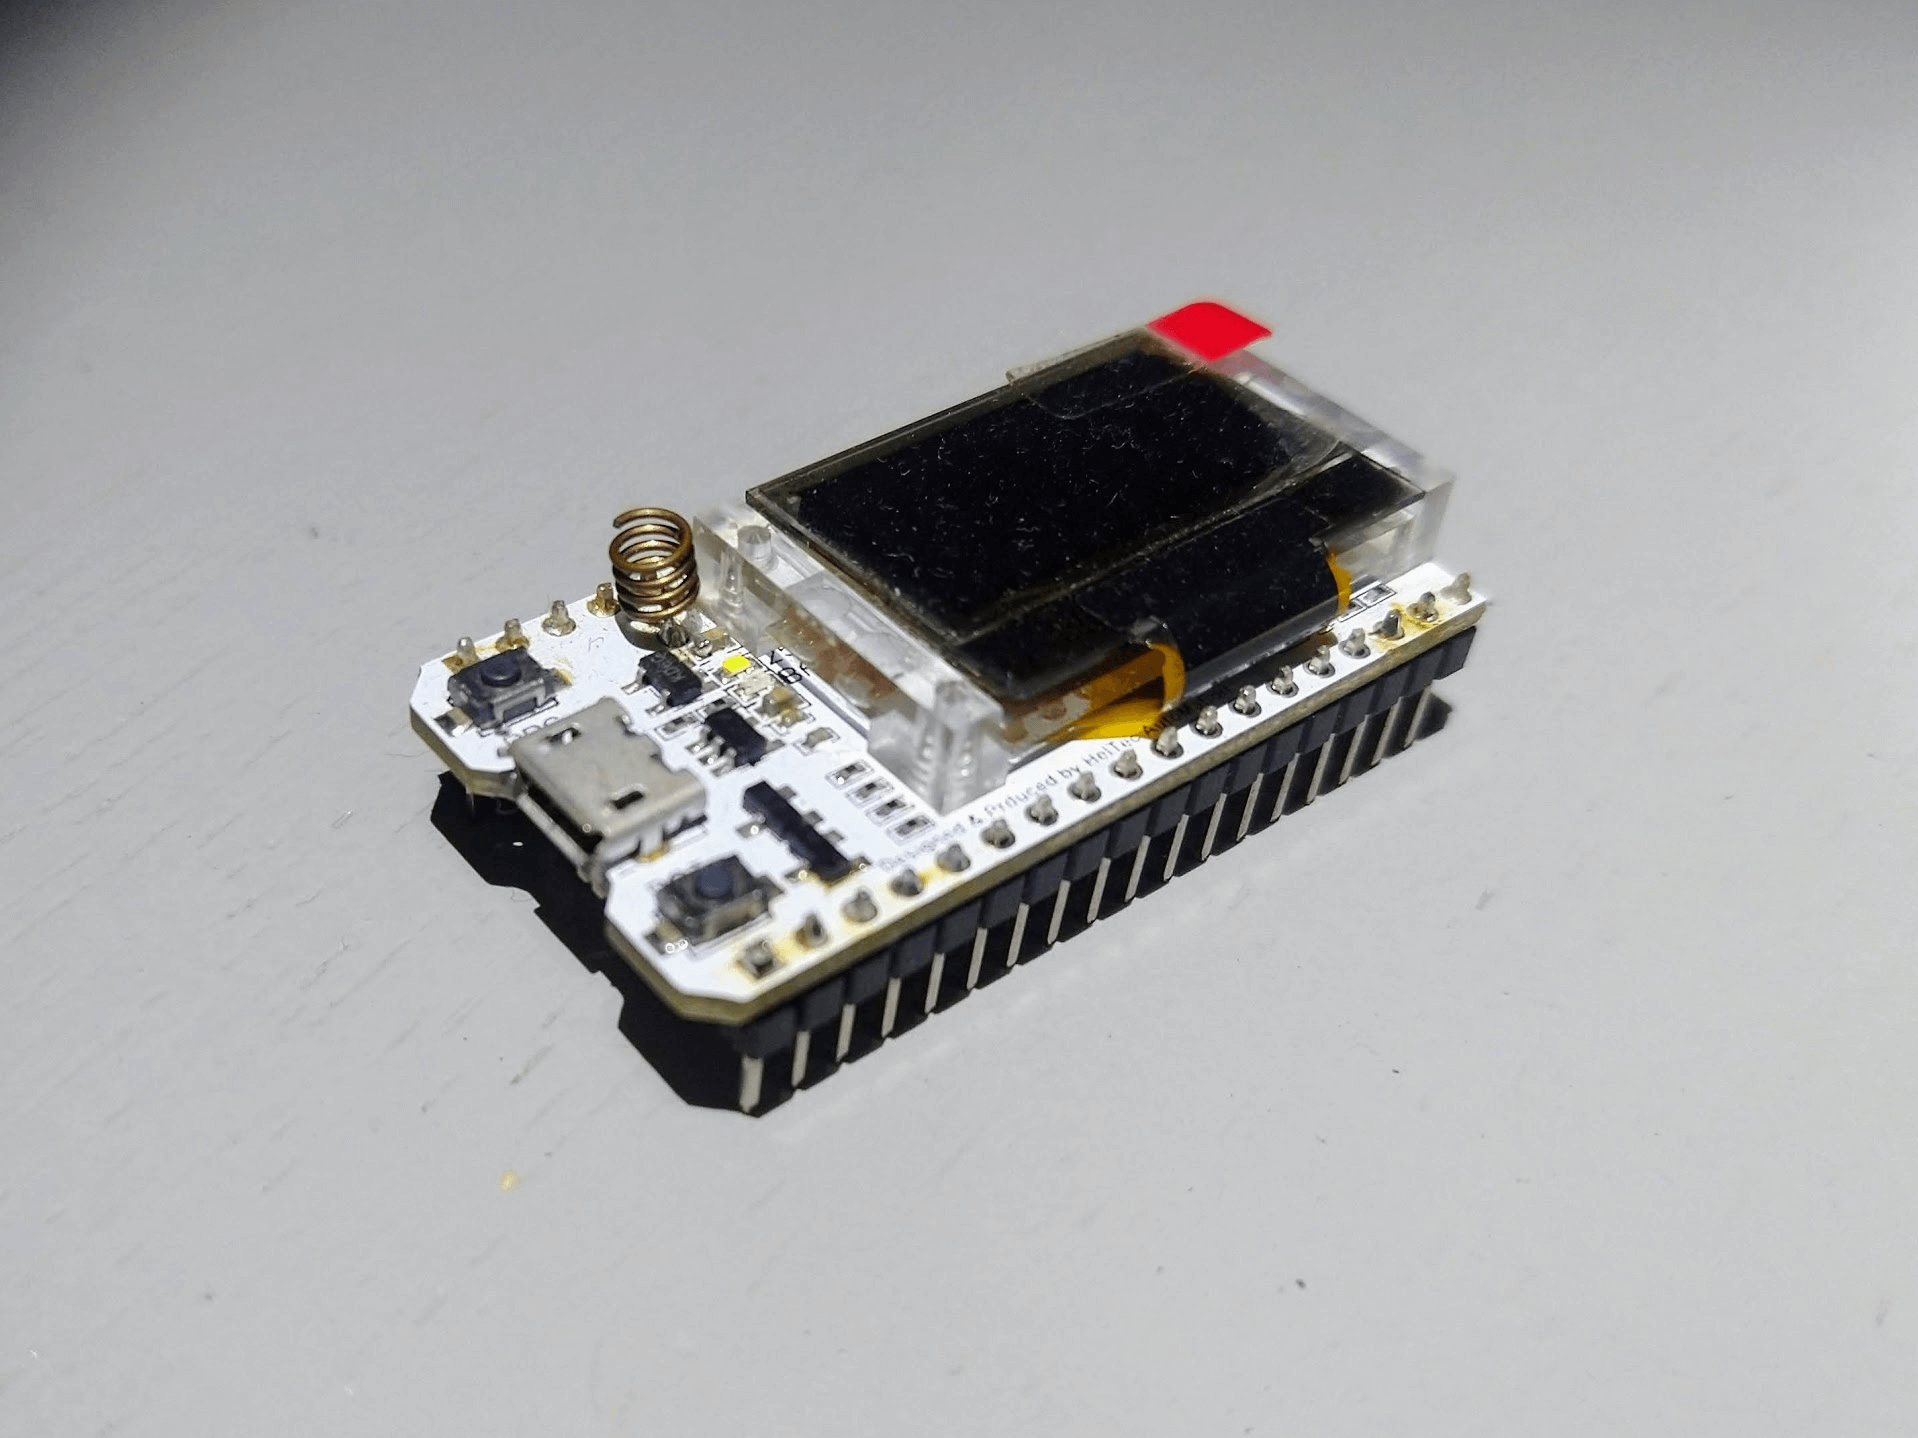
\includegraphics[width=.80\textwidth]{assets/esp32-lora.png} 
  \caption{Foto do ESP32 LoRa da Heltec Automation (autoral).}
  \label{fig:esp32-lora} 
\end{figure}

A configuração do gateway, seu identificador criado pelo servidor e o nome e a senha da rede sem fio que vai ficar conectado, é feita por um ponto de acesso, onde ao liga-lo, ele fornece uma rede sem fio onde é possível acessar seu IP via navegador de Internet, e poder realizar as configurações necessárias.

\begin{figure}[H]
  \centering
  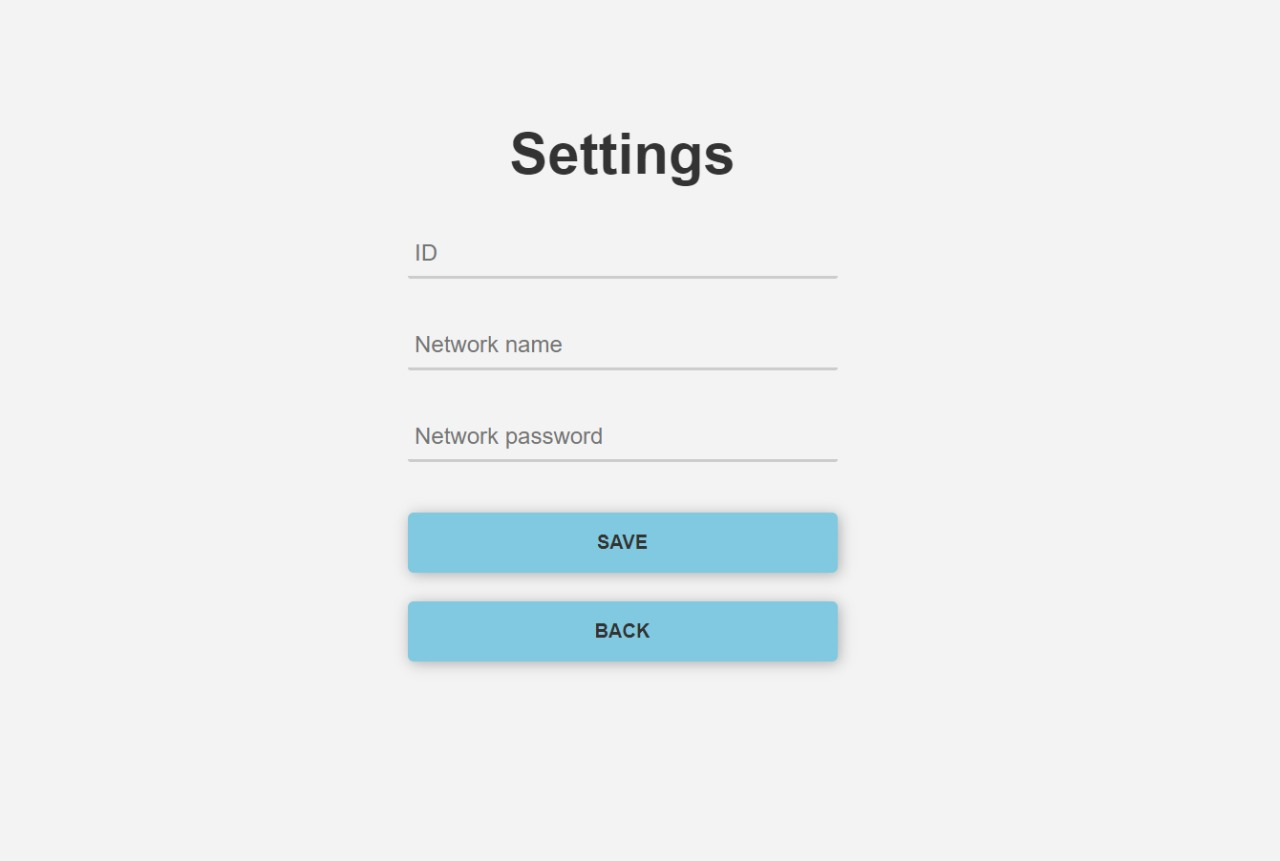
\includegraphics[width=.80\textwidth]{assets/gateway-ap.png} 
  \caption{Página de configuração do gateway (autoral).}
  \label{fig:gateway-ap} 
\end{figure}

% ---
\section{Servidor}
\label{metod:servidor}
Para este projeto, o servidor tem as seguintes responsabilidades: armazenar os dados coletados pelos end-nodes, juntamente com os dados do instituto que está usando a aplicação e dos seus respectivos end-nodes e gateways adquiridos; fornecer rotas para troca de informações com o aplicativo e o gateway, para que possam realizar suas devidas funções.

% ---
\subsection{Padrões de Projetos}
\label{metod:servidor:padroes}
Foi escolhido para desenvolver o servidor, a utilização do Node.js e a linguagem Typescript, se baseando em alguns padrões de softwares, como o Domain-Driven Design (DDD), Test-Driven Development (TDD) e o SOLID visando assim, a construção de um servidor robusto, escalável e de fácil manutenção.

Vale salientar que, esses padrões de softwares, são metodologias de desenvolvimento, e devem ser aplicados de acordo com a demanda da aplicação em construção. Elas são boas práticas, entretanto, dependendo do projeto, alguns pontos podem acabar deixando o processo lendo, e dando pouco benefício, e por isso, nesse projeto, não foi seguido fielmente esses padrões, apenas foi baseado.

Antes de tudo, é preciso definir as regras de negócio básicas do servidor, elas servem para garantir que a aplicação atenda as necessidades esperadas. Para este serviço deve ser possível o usuário se cadastrar, para assim realizar seu \textit{login}, e ter acesso às funcionalidades de cadastrar, editar e remover seus end nodes e seus gateways, além de poder visualizar os dados coletados.

Durante o desenvolvimento de um software, é essencial que a entrega do software funcione corretamente, com qualidade e de acordo com as regras de negócio. Para garantir tais exigências, é importante que se realize testes, tendo em vista identificar possíveis erros antes de chegar aos usuários. Entretanto, realizar testes corretamente é uma tarefa complicada, por isto, existem diversas metodologias, objetivamente facilitar e simplificar os testes dos diferentes componentes de um produto. O TDD é uma dessas metodologias, ela defende o desenvolvimento do teste antes das funcionalidades, garantindo a cobertura completa do código pelos testes.

Junto com o TDD, foi utilizado também o DDD, uma filosofia para auxiliar os desenvolvedores na construção de aplicações complexas de software, ela é referência na organização do código, separando por domínios, de forma isolada. Para poder implementar bem o DDD é preciso definir quais são os domínios da aplicação, analisando as regras de negócio, foi separado em três domínios: end nodes, gateways e usuários.

É preciso também, separar a camada de domínio da aplicação da camada de infraestrutura, a camada de infraestrutura é responsável pelas tecnologias utilizadas para realizar determinada função, por exemplo, a camada de domínio sabe que precisa armazenar os dados dos sensores, mas não é precisar saber onde e nem como, isso é de responsabilidade da camada de infraestrutura.

Para ter uma melhor separação das responsabilidades entre as camadas, é comum utilizar o DDD junto com princípios do SOLID. O SOLID é um acrônimo de 5 princípios da programação orientada a objetos que ajudam o programador a escrever códigos mais limpos, com alta manutenibilidade, separando as responsabilidades e diminuindo acoplamentos.

% ---
\subsection{Banco de Dados}
\label{metod:servidor:db}
É preciso armazenar os dados coletados pelos sensores, para futuras consultas, os dados de transmissão dos pacotes, para utilizar se houver perdas entre as transmissões, e é preciso também, salvar os dados dos usuários e dos seus respectivos produtos cadastrados na plataforma. Tais dados têm suas diferenças, e por isto foi escolhido utilizar banco de dados diferentes para cada um deles.
	
Começando pelos dados coletados pelos sensores e transmitido pelos end-nodes, esses dados são de medidas, coletados com um período curto, e consequentemente, possuem um grande volume. Por isto, foi escolhido utilizar o InfluxDB para armazenar tais dados.

Foi criado duas \textit{measurements} dentro do banco, uma referente aos dados dos sensores e outra aos dados do pacote transmitido, os dois possuindo a mesma  \textit{tag}, o identificador do end node, chamado de endnodeId. Dentro da medida Sensor, foi adicionado dois campos referente a temperatura e umidade do ambiente. Para a medida Package, foi adicionado os campos success, rssi e snr, atributos necessários para saber se o pacote foi entregue com sucesso, a dificuldade de transmitir esse pacote e a relação sinal-ruído. Podemos então ver uma representação do banco na figura \ref{fig:influxdb-model}.

\begin{figure}[H]
  \centering
  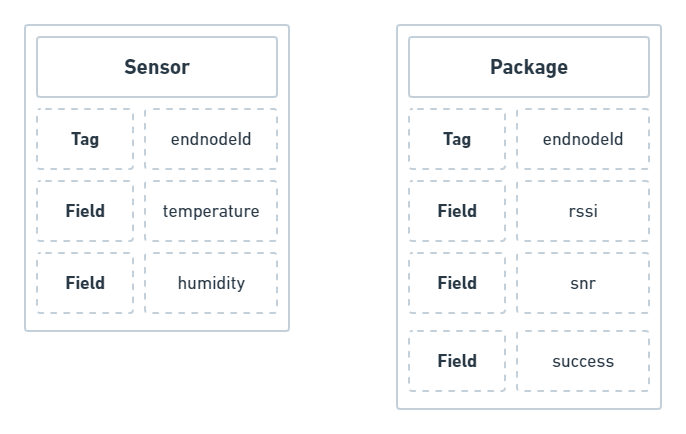
\includegraphics[width=.80\textwidth]{assets/influx-model.png} 
  \caption{Medidas dento do banco de dados InfluxDB (autoral).}
  \label{fig:influxdb-model} 
\end{figure}

Diferentes dos dados que vem dos hardwares, as informações dos usuários e seus dispositivos, não possuem essa demanda alta de escrita e leitura, e mais importante, contém relações entre eles, o que torna banco de dados relacionais uma boa opção para armazenar tais dados. Entre tantos bancos de dados relacionais, foi optado por usar o PostgreSQL por motivos de afinidade.

Cada usuário pode possuir inúmeras gateways e end nodes cadastrados, e cada end node precisa ser vinculado com apenas um gateway. Essas relações entre entre as entidades no postgres representada na figura \ref{fig:postgres-model}, foi pensada olhando tanto para os cenários de pequenos postos de saúde, que tem apenas um local para armazenar seus imunobiológicos, quando para grande hospitais e laboratórios, que pode tem varias salas, com dada sala contendo uma ou mais equipamentos frigoríficos.

\begin{figure}[H]
  \centering
  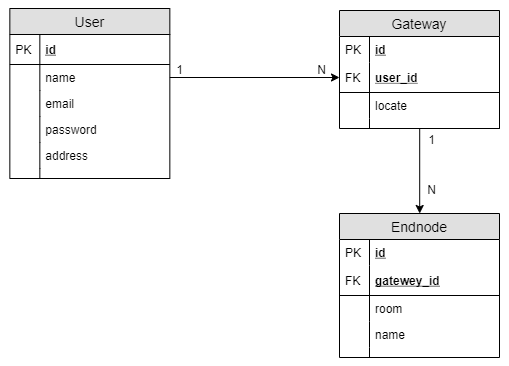
\includegraphics[width=.80\textwidth]{assets/postgres-model.png} 
  \caption{Modelo entidade relacionamento do PostgreSQL (autoral).}
  \label{fig:postgres-model} 
\end{figure}

% ---
\subsection{Containers}
\label{metod:servidor:containers}
Para facilitar o desenvolvimento do servidor, seu deploy e diminuir possíveis problemas por ter várias aplicações rodando na mesma máquina, foi escolhido por conter tantos os bancos de dados quanto a aplicação em si, utilizando o Docker e para facilitar o gerenciamento dos três containers (PostgreSQl, InfluxDB e a aplicação em Node.js), interligando as redes entre eles, foi utilizado o Docker Compose.

Para os bancos de dados, não foi preciso criar as imagens dos containers, dado que são aplicações muito utilizadas e a própria comunidade já oferece algumas opções dependendo da sua finalidade. Entretanto, para a aplicação em si, foi necessário a criação de uma nova imagem, devido algumas configurações extras exigidas pelas tecnologias utilizadas pela aplicação. Tal imagem foi feita baseando-se na versão alpine do node, uma versão mais leve, com apenas as funcionalidades principais.

% ---
\subsection{Deploy}
\label{metod:servidor:deploy}
Entre as opções de servidores na nuvem, foi escolhido por usar a Microsoft Azure para realizar o deploy do servidor. Sua escolha se deu pois a Microsoft oferece uma assinatura para estudantes, o que não teve nenhum custo adicional no desenvolvimento deste protótipo e na realização dos testes.

% ---
\section{Aplicativo móvel}
\label{metod:app}
À necessidade de ter um cliente para que os usuário  possa acessar o histórico de medidas e o gerenciar seus dispositivos, tal cliente poderia ser uma página web, entretanto, tendo em vista o crescimento do uso dos smartphones, tivemos como preferência a criação de uma aplicação móvel, mas especificamente para o sistema operacional Android, devido ao sistema iOS da Apple, restringir seu desenvolvimento para aparelhos da marca, incluindo a necessidade de um computador do mesmo para poder emular um dispositivo móvel com seu sistema operacional.

Tendo em mente as regras de negócios destrinchadas na sessão \ref{metod:servidor:padroes}, a primeira coisa feita foi o desenho das telas utilizando a ferramenta figma, específica para tal tarefa. Ao finalizar os desenhos das telas, partimos para a programação.

Dentre as diversas formas de construir um aplicativo deste porte, a ferramenta escolhida para designar esta função foi o React Native, por motivos de utilizar a mesma linguagem de programação do servidor, typescript, e ter a possibilidade de criar para sistemas iOS futuramente usufruindo do mesmo código.

Pensando na construção de uma aplicação com possibilidades de crescimento altas, foi decidido documentar os componentes que compõem o programa, utilizando a biblioteca Storybook.

\begin{figure}[H]
  \centering
  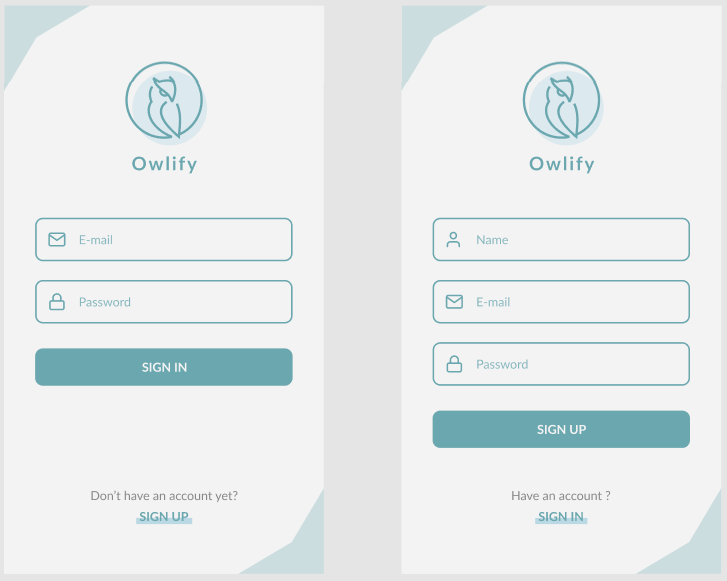
\includegraphics[width=.80\textwidth]{assets/example-app-screens.png} 
  \caption{Desenho das telas de entrar e cadastrar na aplicação (autoral).}
  \label{fig:app-screns-login} 
\end{figure}